
\section{Introduction} % ================== 

Independent of the performace of the previously fit model, we expect unexplained spatial variation in the mean. We assume missing covariates exist, and Tobler's First Law of Geography tells us that things close together in space tend to behave more similarly than things further apart \citep{Tobler1970}. Accordingly, we enhance the model by adding a spatially correlated random effect, giving a Spatial Generalized Linear Mixed Model (SGLMM). The spatial random effect accounts for some of the unexplained spatial variation in the mean, and helps compensate for missing covariates \citep{Banerjee2008}. 

\subsection{Gaussian Random Field} % ================== 

A Gaussian random field (GRF) offers a tractable structure for spatial random effects in a linear model \citep{Gelfand2010}. To define a GRF, first define multivariate Normal random vector $\pmb{w}(\pmb{s})$, for vector of locations $\pmb{s} \in \pmb{D} \subseteq \pmb{R}^{2}$. Define the GRF mean as $\pmb{0}$; and symmetric, positive definite covariance matrix $\Sigma(\pmb{\theta})$, with covariance parameters $\pmb{\theta}$ \citep{Haran2011}. This gives:
$$ \pmb{w}(\pmb{s}) | \pmb{\theta} \sim MVN(\pmb{0}, \Sigma(\pmb{\theta})) $$

Adding a well defined spatial random effect to the GLM linear predictor retools (2) as a {\it spatial} generlatized linear {\it mixed} model (SGLMM). Next we define the GRF covariance structure, $\Sigma(\pmb{\theta})$, that we use in this study.

\subsection{Exponential Covariance}
The spatial random effect $\pmb{w}(\pmb{s})$, defined as a Gaussian random field, requires a spatial correlation structure to. Let $\pmb{w}(\pmb{s})$ be defined as in {\bf 5.1}, with an exponential covariance structure. The following defines the covariance of the random effect at locations $\pmb{s}_{i}$ and $\pmb{s}_{j}$, given as the i,jth element of $\Sigma(\phi, \sigma^{2})$.
\begin{equation}
\Sigma(\phi, \sigma^{2})_{i,j} = \sigma^{2} exp(-||\pmb{s}_{i} - \pmb{s}_{j}||/\phi),
\end{equation}
This definition include the Euclidean distance between $\pmb{s}_{i}$ and $\pmb{s}_{j}$, $||s_{i} - s_{j}||$; scale parameter, $\sigma^{2}$; and range parameter $\phi$.

\subsection{Spatial Generalized Linear Mixed Model}
Adding $\pmb{w}(\pmb{s})$ to the linear predictor in (1) gives the following spatial generalized linear mixed model (SGLMM):
\begin{equation}
\text{logit}(p_{ij}|\pmb{s}_{ij}) = \pmb{X}_{ij}(\pmb{s}_{ij}) \pmb{\beta}_{j} + w(\pmb{s}_{ij}).
\end{equation}

This spatial hierarchical model, containing a latent Gaussian random field, gives $p_{ij}$ a complicated correlation structure. Bayesian statistical methodologies effectively model this structure, and Markov chain Monte Carlo (MCMC) methods can effectively fit spatial models of this kind \citep{Banerjee2014}. Relatively few viable approaches exist for fitting a high dimensional model with this type of complex spatial correlation. High dimensionality for this type of spatial model induces significant computational cost, referred to as the `Big N problem' \citep{Lindgren2011}.

\subsection{The ``Big N'' Problem}

To consider the SGLMM, recall the multivariate Normal probability distribution function, in this case for $\pmb{w}$.

$$ f(\pmb{w}) = \frac{1}{(2\pi)^{n/2}|\Sigma|^{1/2}} \text{exp}\{ -\frac{1}{2}\pmb{w}'\Sigma^{-1}\pmb{w} \}$$

Note that $|\Sigma|^{1/2}$ denotes the square root of the determinant of the $n \times n$ covariance matrix, and $\Sigma^{-1}$ denotes its inverse. These two elements of the MVN distribution lead to a sometimes prohibitive computational cost. To understand this cost, we first define ``big oh'' notation. 

For a sequence of two increasing functions $f(n)$ and $g(n)$, we say ``$f(n)$ is big `oh' $g(n)$ as n goes to infinity,'' or $f(n) = O(g(n))$ as $n \rightarrow \infty$, if and only if there exists some $n_{0}$ and a positive real number M such that
  $$|f(n)| \leq M \cdot |g(n)| \text{ for all } n \geq n_0 $$
In our situation, then, we know that the computational costs of fitting a SGLMM increase at a rate of $\mathcal{O}(n^{3})$ \citep{Finley2009}. Therefore, define t(n) as time required for SGLMM model fitting, and we have:
$$t(n) \leq M \cdot n^{3} \text{ as } n \rightarrow \infty.$$
In less technical terms, this means the upper bound on the amount of time required for model fitting increases at the same rate as $n^{3}$. To understand why, referring back to the MVN pdf, and notice (i) the $n \times n$ covariance matrix inverse and, (ii) the determinant. These calculations, required in every iteration of an MCMC algorthm, account for the $\mathcal{O}(n^{3})$ rate of increase, prohibitively slow model fitting, and the ``Big N'' problem.

\subsection{Approaches}
With the considerable compuatational costs just described in placed, we used three approaches to fitting SGLMMs in practical time frames.

\begin{enumerate}
\item Computational optimization in Bayesian computing software Stan.
\item Dimension reduction with Predictive process models, implemented in the R package \verb|spBayes|.
\item Integrated Nested Laplace Approximations with Stochastic Partial Differential Equations, implemented in the R package \verb|INLA-R|.
\end{enumerate}

% Note that the ultimate goal of this research is practical, real-time applications for baseball fans, broadcasts, players, scouts, and teams. Therefore, model fitting speed matters on a finer time scale than academic research demands.  

The first two approaches rely on what has become the dominant Bayesian model fitting algorthm, Markov chain monte carlo, and the subject of the next section.

\section{Markov Chain Monte Carlo}

Elementary Bayesian models sometimes yield closed form posterior distributions, but more complex models rarely do\footnote{The details of this section rely heavily on the presentation of MCMC algorithms in \cite{Banerjee2014}}. In these cases, Markov chain simulations, usually called Markov Chain Monte Carlo (MCMC), offer an iterative procedure that converges to the true posterior distribution. This class of procedures presents its own challenges, and even weaknesses.  Nevertheless, with sufficient computing power and time MCMC often provides the desired posterior distributions. This holds true for a breadth of problems, hence MCMC's widespread use \cite{Banerjee2014}. The MCMC solution presents empirically, as draws from the posterior distribution of interest, rather than as a closed form. 

Markov chain properties supply the fundamental theoretical elements of MCMC. A sequence of possibly multivariate random variables $\pmb{X}_{1}, \pmb{X}_{2}, \hdots$ with the Markov property---the distribution of $\pmb{X}_{n+1}$ given $\pmb{X}_{1}, \pmb{X}_{2}, \hdots , \pmb{X}_{n}$ depends only on $\pmb{X}_{n}$---defines a Markov chain. MCMC algorithms use carefully constructed Markov chains that possess the necessary technical properties to assure an equilibrium distribution \citep{Brooks2011}. In fact, these chains are constructed so that they converge to an equilibrium distribution equivalent to the posterior distribution of interest.

Both Bayesian estimation programs used in this chapter use the Metropolis sampling algorithm, one of the most popular MCMC algorithms. \verb|Stan| uses HMC sampling and a ``Metropolis reject step'' \citep{STANtheMan}. \verb|spBayes|, for our purposes, uses a ``Metropolis-within-Gibbs'' sampler \citep{Finley2013}.

\subsection{Gibbs Sampler}
In high dimensional problems that are now common, the Gibbs Sampler achieves success, in part, because it iteratively reduces the dimension of the problem. To understand how, and give the algorithm, define parameter vector $\pmb{\theta} = (\theta_{1}, \dots, \theta_{k})'$, and assume we can draw samples from $p(\theta_{i}|\theta_{j \neq i},y)$ directly, or using the Metropolis algorithm described in the next section . The Gibbs sampler proceeds with the following steps, for iterations $(t \in 1:T)$ \citep{Banerjee2014}. 
        \begin{itemize} 
        \item Step 1: draw $\theta_{1}^{t}$ from $p \left( \theta_{1}|\theta_{2}^{t-1}, \theta_{3}^{t-1},\dots,\theta_{k}^{t-1},\pmb{y} \right)$ 
        
        \item Step 2: draw $\theta_{2}^{t}$ from $p \left(\theta_{2}|\theta_{1}^{t}, \theta_{3}^{t-1},\dots,\theta_{k}^{t-1},\pmb{y} \right)$ \\
        $\vdots$ \\ 
        \item Step k: draw $\theta_{k}^{t}$ from $p \left( \theta_{k}|\theta_{1}^{t}, \theta_{3}^{t},\dots,\theta_{k-1}^{t},\pmb{y} \right)$ 
        \end{itemize} 
With certain regularity conditions satisfied, as they are in MCMC usage, this structured sequence of draws converges to draws from the true posterior distribution $p(\pmb{\theta}|\pmb{y})$ \citep{Banerjee2014}. 

\subsection{Metropolis Algorithm} 
\citep{Banerjee2014}
Often we don't know the closed form for a particular target distribution; possible targets include the conditional of a single MCMC iteration, or the full Bayesian posterior posterior. However, we always know the target distribution up to a proportionality constant. Recall the fundamental Bayesian proportionality, for observation vector $\pmb{y}$, and parameter vector $\theta$,
$$p(\pmb{\theta}|\pmb{y}) \propto f(\pmb{y}|\pmb{\theta})p(\pmb{\theta}).$$
We clearly see the kernal---the portion that contains the parameters of interest. Call the kernal $h(\pmb{\theta})$. The Metropolis algorithm uses $h(\pmb{\theta})$ to draw conditional sample from  iteration to iteration. These full conditional iterative draws, $p(\theta_{i}|\pmb{\theta}_{-i})$, effectively reduce a possibly high dimensional problem to a series of lower dimension problems. Before the algorithm procedds, one must specify a candidate density, $q(\pmb{\theta}_{t}|\pmb{\theta}_{t-1})$, such that:
  \begin{enumerate}
  \item The candidate density support contains all possible values of $\pmb{\theta}_{t}$ and $\pmb{\theta}_{t-1}$; 
  \item $q(\pmb{\theta}_{t}|\pmb{\theta}_{t-1}) = q(\pmb{\theta}_{t-1}|\pmb{\theta}_{t})$; symmetric.
  \item We can readily draw samples from $q(\pmb{\theta}_{t}|\pmb{\theta}_{t-1})$.
  \end{enumerate}
Next, the Metropolis requires an initial value, call it $\pmb{\theta}_{0}$, for $\pmb{\theta}$. Then, for $(t \in 1:T)$, where T is some prescribed number of iterations, the Metropolis algorithm proceeds as follows.
\begin{enumerate}
\item Generate candidate value of $\pmb{\theta}$, call it $\pmb{\theta}^{*}$, from $q(\pmb{\theta}^{*}|\pmb{\theta}_{t})$.
\item Compute the ratio of kernals,
$$ r=h(\pmb{\theta}^{*})/h(\pmb{\theta}^{t-1}) = \text{exp}[\text{log }h(\pmb{\theta}^{*}) - \text{log }h(\pmb{\theta}^{(t-1)}). $$
\item If $r \geq  1$, set $\pmb{\theta}^{t} = \pmb{\theta}^{*}$; \\
            If $r < 1$, set 
            \[ 
            \pmb{\theta}^{t} = 
            \begin{cases} 
            \pmb{\theta}^{*} \text{ with probability r} \\
            \pmb{\theta}^{(0)} \text{ with probability 1 - r} \\
            \end{cases}
            \]
  \end{enumerate}
  
In this way, the Metropolis algorithm, typically in combination with the Gibbs sampler, enables the MCMC algorithm to iteratively work its way to the posterior distribution of interest.

% \subsection{Evaluate Inverse? Yes.}
% \begin{itemize}
% \item logit\{EY(s)\} = $\pmb{X}(s)\pmb{\beta} + Z(s)$, with $Z(s) \sim MVN\{\pmb{0}, \Sigma_{s}\}$
% \item $f(\pmb{\beta}, \phi, \sigma^{2}, \pmb{Z}|\pmb{Y}) \propto f(\pmb{Y}|\pmb{\beta}, \phi, \sigma^{2}, \pmb{Z})f(\pmb{\beta})f(\pmb{Z}|\phi, \sigma^{2})f(\phi)f(\sigma^{2})$
% \item M-H proposal, iteration i: $Z_{10,i}$
% $$ r = \frac{ f(Z_{10,i}|\pmb{Z}_{1:9,i},\pmb{Z}_{11:n,i-1}, \pmb{\beta}_{i-1}, \phi_{i}, \sigma^{2}_{i})}{f(Z_{10,i-1}|\pmb{Z}_{1:9,i},\pmb{Z}_{11:n,i-1}, \pmb{\beta}_{i-1}, \phi_{i}, \sigma^{2}_{i})} $$
%  
% \item Note: $f(z_{1}, z_{2}, z_{3}|\pmb{Y}) = f(z_{1}|z_{2},z_{3},\pmb{Y})f(z_{2},z_{3}|\pmb{Y})$. So... $$r \propto \frac{f(\pmb{Y}|\pmb{\theta}_{i})f(\pmb{\beta})f(Z_{10,i}|\pmb{Z}_{1:9,i},\pmb{Z}_{11:n,i-1}, \phi_{i}, \sigma^{2}_{i})f(\pmb{Z}_{1:9,i},\pmb{Z}_{11:n,i-1}|\phi_{i}, \sigma^{2}_{i})f(\phi)f(\sigma^{2})} {f(\pmb{Y}|\pmb{\theta}_{i-1})f(\pmb{\beta})f(Z_{10,i-1}|\pmb{Z}_{1:9,i},\pmb{Z}_{11:n,i-1}, \phi_{i}, \sigma^{2}_{i})f(\pmb{Z}_{1:9,i},\pmb{Z}_{11:n,i-1}|\phi_{i}, \sigma^{2}_{i})f(\phi)f(\sigma^{2})}$$
% 
% $$ r \propto \frac{f(\pmb{Y}|\pmb{\theta}_{i})f(Z_{10,i}|\pmb{Z}_{1:9,i},\pmb{Z}_{11:n,i-1}, \phi_{i}, \sigma^{2}_{i})}
% {f(\pmb{Y}|\pmb{\theta}_{i-1})f(Z_{10,i-1}|\pmb{Z}_{1:9,i},\pmb{Z}_{11:n,i-1}, \phi_{i}, \sigma^{2}_{i})} $$
% 
% \item And $f(\pmb{Z})$, $f(Z_{i}|\pmb{Z}_{-i})$, etc. are $MVN\{\cdot,\Sigma^{*}\}$, where $\Sigma^{*}$ either is, or is some function of, $\Sigma_{\pmb{s}}$; with PDF kernal containing $\Sigma_{\pmb{s}}^{*-1}$, (containing $\phi_{i}, \sigma^{2}_{i})$.
% \end{itemize}
        
\section{Optimization in Stan} % =================

An MCMC algorithm involving a difficulte-to-sample-from distribution requires a proposal generating mechanism of some kind. Often, a random walk distribution, or some othe accessible distribution plays this role. Stan, however, uses a proposal mechanism that originated in physics, Hamiltonian Monte Carlo (HMC), to generate proposals for the Metropolis reject step. The proposal mechanism influences key components of an MCMC algorithm greatly, including sampling correlation and distribution convergence. Mixing, or the degree to which proposals explore the parameter support, and acceptance rates of proposals play central roles. For example, insufficient mixing and low acceptance rates delay, or even prevent, convergering to the posterior. An acceptance rate too high signals insufficient mixing and highly correlated draws. In Stan's MCMC, HMC balances the proposal mechanism demands well.

\subsection{Hamiltonian Monte Carlo}% =================

\footnote{The history and physics presented here follows the presentation in \cite{Neal2011}.}Trying to understand molecular states, \cite{Metropolis1953} created MCMC for ``fast machines.'' Later, modeling molecular motion as a deterministic process, \cite{Alder1959} introduced {\it Hamiltonian dynamics} as an alternate representation of Newtonian mechanics. Almost 30 years later, \cite{Duane1987} combined the two to create ``hybrid Monte Carlo,'' used to simulate quantum mechanical processes. Over time, the name morphed into {\it Hamilton} Monte Carlo (HMC). Eventually, \cite{Neal1996} used HMC methods for explicitly statistical applications, studying neural networks.

HMC works by reframing the variables and distribution of interest as though part of a physical system. From a physics standpoint, position and momemtum completely characterize an object in a well defined three dimensional physical space. For HMC, the variables of interest play the role of position variables, and HMC artificially introduces auxiliary Gaussian variables to serve as momentum variables. Simple updates for the auxiliary momentum variables generate, via a system of differential equations, proposals for Metropolis updates to the more important position variables (which represent the variabls of interest). The differential equation solutions estimate trajectories of the hypothetical physical object, which will then occupy a new position after a time step of some chosen duration. This crafty formulation enables distant, yet high probability, proposals for the variables of interest. Note that this contrasts favorably, in terms of mixing, to the random walk proposal generation process commonly used for Metropolis updates.

\subsubsection{Hamilton Equations for MCMC} % =================

Let d-dimensional function and position vector $q(t)$ depend on time $t$ (dimension of $q(t)$ equal to dimension of parameter of interst); and $U(q(t))$ represent the potential energy at time $t$. Let $p(t)$ give the d-dimensional momentum at time $t$, and $K(p(t))$ represent kinetic energy at time $t$. Then the Hamilton equation,
\begin{equation}
H(q(t),p(t)) = U(q(t)) + K(p(t)),
\end{equation}
measures the total energy of a system. 

For HMC applications, we let the potential energy, $U(q)$, be minus the log of the probability density function of interest, plus any convenient constant\footnote{We omit $t$ for clarity of presentation, here and elsewhere, but position and momentum remain functions of time $t$.}. Typically, HMC procedures define $p$ as a d-dimensional zero mean Gaussian with covariance matrix M, and $K(p)$ as minus the log of the multivariate Gaussian probability density function. This gives:
\begin{align}
H(q,p) = -\text{log}f_{q}(q) + p^{T}\pmb{M}^{-1}p/2.
\end{align}
This clever formulation provides relatively simple partial derivatives for calculating the change in position and momentum over time. For $i = 1,\dots, d$:
\begin{align}
\frac{d q_{i}(t)}{dt} &= \frac{\partial H}{\partial p_{i}}, \\
\frac{d p_{i}(t)}{dt} &= -\frac{\partial H}{\partial q_{i}}.
\end{align}
Substituting in Hamilton's equation (5) and simplifying gives
\begin{align}
\frac{d q_{i}(t)}{dt} &=  [\pmb{M}^{-1}p]_{i} \\
\frac{d p_{i}(t)}{dt} &= \frac {\partial \left[ \text{log}f_{q}(q) \right]}{\partial q_{i}}
\end{align}
The solutions to these two differential equations, $q(t)$ and p(t) such that (8) and (9) hold, give the instantaneous rate of change of position and momentum at time t. 

This structure and the ``leapfrom method'' combine to for the HMC method. The ``leapfrog method'' calculates changes in the Hamilton through small time steps, which involvs discretizing the continuously defined Hamilton equation using Taylor Series approximations \citep{Neal2011}. In summary, the algorithm readily samples from K(p), the kinetic energy as a function of momentum, chosen for its sampling ease and simplicity; and calculates new U(q) values, the potential energy as a function of position, and also the variables of interest. This methods yields high probability, yet well mixed, Metropolis proposals.

% \subsubsection{MCMC Using Hamiltonian Dynamics } % ======
%   \begin{itemize}
%   \item Postion (q) (or momentum (p)) at $t_{0}$ plus time step times rate of change of position (q) (momentum (p)) variable at $t_{0}$ \citep{Neal2011}
%   \item Leapfrom Method does half step for momentum (p), full step for postion (q), other half step for momentum (p). Damn good.
%   \end{itemize}

\subsection{Optimizing in Stan} % =================
Certain program specific coding techniques can mitigate `Big n' computational burdens. We focused on these techniques, as well as other techniques aimed to encourage model convergence, in the first stage of our modelling efforts. We describe the techniques we used, in Stan here, and include the complete .stan script in Appendix A for reference. 

\subsubsection{Bayesian Techniques} % =================

Stan permits users to omit prior distributions for parameters, but interprets non-inclusion as a non-informative, uniform prior. However, \cite{Gelman}, the first Stan developer, pointed out in correspondence that the exponential covariance range parameter, $\phi$ in equation 2.1, requires an informative prior for model identifiability, or uniqueness \citep{Gelman2014}. In this vein, \cite{Trangucci} recommended a sharp tailed prior distribution for range parameter $\phi$, such as the normal or log-normal, to act as soft upper and lower bound constraints. Even further, for practical computing time and convergence considerations, complex models such as spatial hierarchical models require proper priors for all of the $\beta$ coefficients \citep{Trangucci}. Indeed, using the previous GLM coefficient estimates to inform coefficient prior distributions indeed sped up computation considerably.

\subsubsection{Computational Techniques} % =================
For speed and efficiency, the Stan Users Manual recommends pure matrix algebra and vectors, over `for loops' and scalars \cite{STANtheMan}. For example, 
\begin{verbatim}
hit ~ bernoulli_logit(X*beta + Z)
\end{verbatim}
runs faster than
\begin{verbatim}
for (n in 1:N)
        hit[n] = bernoulli_logit(X[n]*beta[n] + Z[n])
\end{verbatim}
Notice that $N \times 1$ column vectors \verb|hit|, \verb|beta|, and \verb|Z| replace scalars \verb|hit[n]|, \verb|beta[n]|, and \verb|Z[n]|; and $N \times p$ matix \verb|X| replaces $1 \times p$ row vector \verb|X[n]|.

\cite{Trangucci} also suggested a QR factorization on covariate matrix $\pmb{X}$, in the linear predictor, to increase computational efficiency. A QR factorization consists of factoring an $n \times p$ matrix into the product of an $n \times p$ orthogonal matrix $\pmb{Q}$ and a $p \times p$ upper triangular matrix $\pmb{R}$, such that $\pmb{X} = \pmb{QR}$. 
\begin{align}
\pmb{X} &= \pmb{QR} \\
\pmb{X \beta} &= \pmb{QR \beta}
\end{align}
This necessitates a reparameterization for model fitting. To this end, let $\pmb{\theta} = \pmb{R \beta}$, so that $\pmb{\beta} = \pmb{R^{-1}\theta}$, which gives
\begin{align}
\pmb{X \beta} &= \pmb{Q \theta}, \text{ and } \\
\text{logit}(p_{ij}|\pmb{s}_{ij}) &= \pmb{Q}_{ij}(\pmb{s}_{ij}) \pmb{\theta}_{j} + w_{ij}.
\end{align}
We incorporate prior information about $\pmb{\beta}$ in the $\pmb{\theta}$ prior distributions. Consider non-informative prior distributions on $p$ dimensional parameter vector $\pmb{\beta}$,
$$ \pmb{\beta} \sim N(\pmb{0}, \sigma^{2}\pmb{I}_{p}), $$
with $p \times p$ identity matrix $\pmb{I}_{p}$; and $p \times 1$ zero vector $\pmb{0}$. Notice the intended variance of the non-informative prior must be modified for $\pmb{\theta}$.
\begin{align}
\text{Var}(\pmb{\theta}) &= \text{Var}(\pmb{R \beta}) \\
&= \pmb{R}\text{Var}(\pmb{\beta})\pmb{R}' \\
&= \pmb{R}\sigma^{2}\pmb{I}_{p}\pmb{R}' \\
&= \sigma^{2} \pmb{R}\pmb{R}'
\end{align}

Next, we add noise to the covariance matrix diagonal with the following snippet of code.
\begin{verbatim}
for (n in 1:N)
  Sigma[n, n] = Sigma[n, n] + 1e-6;
\end{verbatim}
The stan function \verb|cov_exp_quad(...)| assembles the covariance matrix, and the added diagonal noise guarantees that it remains numerically positive-definite \cite{Trangucci2017}. This reduces wasted MCMC iterations because \verb|cov_exp_quad(...)| can generate numerically non-positive-definite matrices when operating at high dimensions.

Finally, \cite{Carpenter} recommended a Cholesky decomposition and tactical reparameterization, noting the efficiency of a vectorized scalar approach.
\begin{verbatim}
L = cholesky_decompose(Sigma);  
Z ~ normal(0, 1);  
Z_mod = L * Z; 
hit ~ bernoulli_logit(Q*theta + Z_mod);
\end{verbatim}
The first line performs a Cholesky decomposition on the covariance matrix \verb|Sigma|. A Cholesky decomposition factors symmetric matrix \verb|Sigma| such that $\Sigma = \text{\pmb{LL}}'$. Line 2, ``vectorized scalar'' \verb|Z ~ normal(0, 1)| generates $n$ standard normal random variables, by reusing \verb|normal(0, 1)| for every element of \verb|Z|. These two lines remove the dependence of random vector \pmb{Z}, which must be generated, on unknown parameters \cite{Trangucci2017}. The third line, \verb|Z_mod = L * Z|, uses \verb|Z| to give \verb|Z_mod| the desired distribution. Note that $\text{Var}(\text{\pmb{LZ}}) = \text{\pmb{L}} \text{I}_{n}\text{\pmb{L}}' = \Sigma$, so that $\pmb{LZ} \sim N(\pmb{0}, \Sigma)$ as desired.

\subsubsection{Results}

In initial model fitting, using a test data set of n = 25 observations, to sample one 500 sample chain required approximately 50 seconds of computing time. Using the Cholesky decomposition described above reduced this time to 26 seconds. Proper priors on covariance parameters and noise on the covariance diagonal drastically reduced the number of numerical/sampling errors and warning messages, shaving another couple seconds off the computing time. Putting proper, non-informative priors on all elements of $\pmb{\beta}$ reduced computing time for n=25 observations to approximately 5 seconds. However, scaling up a bit, n=500 observations required approximately 100 minutes (6000 seconds). Increasing the observations by a factor of 100 increased the computing time by a factor of 1200. The $\pmb{QR}$ decomposition yielded further gains; n = 1000 observations required about an hour. As a reference point, the same number of observations at this stage required about six seconds. Despite these improvements, Stan efforts concluded with n = 2000, when an overnight MCMC run yielded only 350 of 500 samples.

The ``big N'' problem clearly hindered our modeling effort. Next, we looked to a dimension reduction approach developed for, and subsequently used in, forestry and ecology.

\section{Dimension Reduction with Predictive Process Models} % =========

Predictive process models (PPMs) provide a method for attempting to circumvent the ``big N problem'' in the case of Bayesian hierarchical models with latent Gaussian random effects. Numerous general approaches exist for this task, with at least several methods for each approach. For example, for data on a regular lattice \cite{Fuentes2007} and \citep{Paciorek2007} use a spectral representation of the covariance function and Fourier transforms. Others developed ``covariance tapering,'' whereby the small values in the covariance matrix are set to zero \citep{Furrer2006}, \citep{Kaufman2008}. Various compuational approximations exist, and we explore one in Section 2.5 \citep{Rue2009}, but others exist \citep{Stein2004}, \citep{Eidsvik2014}, \citep{Aune2014}. Still more apply exact methods to a simplified, lower rank version of the original model. \citep{Cressie2008}, \citep{Higdon2002}, \citep{Eidsvik2012}. Our next approach belongs to this last category. 

Predictive process models provide a competitive modeling approach with computational advantages specifically for hierarchical models with a Gaussian random field (GRF) at the second level of specification \citep{Banerjee2008}. Latent GRFs prove challenging because they are only implicitly observed, through a binomial response in our case. This means the GRF parameters (hyperparameters) and their prior distributions comprise the third level of the hierarchical model. Gaussian PPMs achieve dimension reduction by projecting the original process onto a lower dimensioned subspace, at a set of locations called knots \citep{Banerjee2008}. 

\subsection{PPM Procedure}

Consider again the SGLMM (5), and Gaussian random field $\pmb{w}(\pmb{s})$.
\begin{align}
\text{logit}(p_{ij}|\pmb{s}_{ij}) &= \pmb{X}_{ij}(s_{ij}) \pmb{\beta}_{j} + w(\pmb{s}_{ij}) \\
\pmb{w}(\pmb{s}) | \pmb{\theta} &\sim \text{GRF}(\pmb{0}, \pmb{C}(\pmb{\theta}))
\end{align}

Define (20) as in (5), and (21) shows $n \times 1$ vector of random effects $\pmb{w}$ at locations $\pmb{s}$, conditioned on covariance parameters $\pmb{\theta}$, constitutes a GRF. Let $n \times 1$ zero vector $\pmb{0}$ be the stationary GRF mean, with $n \times n$, symmetric, positive-definite covariance matrix $\pmb{C}(\pmb{\theta})$. Let $C(\pmb{s}_{i}, \pmb{s}_{j}; \pmb{\theta})$ denote the covariance of random effects at locations $\pmb{s}_{i}$ and $\pmb{s}_{j}$, so that $C(\pmb{\theta}) = [C(\pmb{s}_{i}, \pmb{s}_{j}; \pmb{\theta})]_{i,j=1}^{n}$.

To define the PPM, start with knot locations. Let $\pmb{S}^{*} = \{\pmb{s}_{1}^{*}, \dots, \pmb{s}_{m}^{*}\}$ be a set of $m < n$ chosen knot locations, which may or may not be a subset of observed locations. We denote knot location random effects with $m \times 1$ vector $\pmb{w}^{*} = \left[w(\pmb{s}_{i}^{*})\right]_{i=1}^{m}$, and the $m \times m$ knot covariance matrix and its elements as $\pmb{C}^{*}(\pmb{\theta}) = \left[C(\pmb{s}_{i}^{*}, \pmb{s}_{j}^{*})\right]_{i,j = 1}^{m}$. The knot random effects form a distinct $m$-dimensional GRF.
\begin{equation}
\pmb{w}^{*}|\pmb{\theta} \sim \text{GRF}\{\pmb{0}, \pmb{C}^{*}(\pmb{\theta})\}
\end{equation}
The predictive process modelling procedure uses the $m$ selected knots, the covariance structure of the parent process, and kriging to interpolate $w$ at site $\pmb{s}_{0}$ \citep{Schabenberger2004}; See Appendix ?? for kriging details. Let $\tilde{w}(\pmb{s}_{0})$ represent this interpolated random effect, and let $\pmb{c}(\pmb{s}_{0};\pmb{\theta}) = \left[C(\pmb{s}_{0}, \pmb{s}_{j}^{*}; \pmb{\theta})\right]_{j = 1}^{m}$ be an $m \times 1$  covariance vector giving the covariance of the $\pmb{s}_{0}$ random effect with the knot random effects.
\begin{align}
\tilde{w}(\pmb{s}_{0}) &= E[w(\pmb{s}_{0})|\pmb{w}^{*}] \\ 
&= \pmb{c}^{T}(\pmb{s}_{0};\pmb{\theta}) \cdot \pmb{C}^{*-1}(\pmb{\theta}) \cdot \pmb{w}^{*}
\end{align}
For a GRF, the weights of linear combination (24) minimize the squared error loss function among all linear predictors \citep{Schabenberger2004}; and notice that the linear combination varies spatially. Accordingly, predictive process $\tilde{w}(\pmb{s})$ defines another GRF and covariance matrix.
\begin{align}
\tilde{\pmb{w}}(\pmb{s}) &\sim \text{GRF}\{0, \tilde{C}(\cdot)\} \\
\tilde{C}(\pmb{s}, \pmb{s}'; \pmb{\theta}) &= \pmb{c}^{T}(\pmb{s};\pmb{\theta}) \cdot \pmb{C}^{*-1}(\pmb{\theta}) \cdot \pmb{c}(\pmb{s}';\pmb{\theta})
\end{align}
To reiterate, $m \times 1$ vector $\pmb{c}(\pmb{s};\pmb{\theta}) = \left[C(\pmb{s}, \pmb{s}_{j}^{*})\right]_{j = 1}^{m}$ gives the covariance of the random effect at $\pmb{s}$ with knot random effects. Finally, the predictive process model:

\begin{equation}
\text{logit}(p_{ij}|\pmb{s}_{ij}) = \pmb{X}_{ij}(\pmb{s}_{ij}) \pmb{\beta}_{j} + \tilde{w}(\pmb{s})
\end{equation}

\subsection{Improved Predictive Process Models}


\section{Integrated Nested Laplace Approximations with Stochastic Partial Differential Equations} % =================
Integrated Nested Laplace Approximation (INLA), a mathematically intensive and computationally geared approximation technique, works well for Bayesian hierarchical models with latent Gaussian {\bf markov} random fields (GMRFs) \citep{Rue2007}. A GMRF, by virtue of its sparse precision matrix, enables INLA's orders of magnitude faster approximation method. However, to use INLA for continuous domain spatial models with latent Gaussian random fields (GRFs), one must represent the GRF as a GMRF; and stochastic calculus provides a link. A particular stochastic partial derivative of a Matern GRF equals a Gaussian random field white noise process. This identity provides a platform on which to approximate a Matern GRF with a GMRF, in the form of a piecewise linear basis representation. The discrete representation consists of deterministic basis functions, defined by a triangulation of the domain, and GMRF weights. The basis representation has a sparse precision matrix, and thus qualifies for the INLA approximation and its computational advantages. Scientists use this GRF to GMRF translation process---projecting the SPDE onto the basis representation---known as Finite Element Method, extensively in other fields. 
\subsection{Gaussian Markov Random Fields}

\subsection{Stochastic Partial Differential Equation (SPDE)} 

The exponential convariance function is a member of the larger Matern family, defined by the following covariance function.
$$\text{C}(h) = \frac{\sigma^{2}}{2^{\nu - 1}\Gamma(\nu)}(\kappa h)^{\nu}K_{\nu}(\kappa h)$$
This parameterization includes range parameter $\kappa > 0$, smoothness parameter $\nu > 0$, scale parameter $\sigma^{2}$, and modified Bessel function $K_{\nu}(\cdot)$ \citep{Schabenberger2004}. While $\nu = 1/2$ defines the exponential covariance function, \cite{Whittle1954} declared Matern($\nu = 1$) the ``elementary correlation'' function in two dimensions. Both functions yield a similarly decaying-with-distance spatial covariance, but a Matern random field solves the following SPDE \citep{Whittle1954}.
$$(\kappa^{2} - \Delta)^{\alpha/2}x(\pmb{s}) = \mathcal{W}(\pmb{s}),$$ 
This includes $\Delta = \sum_{i=1}^{d} \frac{\partial^{2}}{\partial x_{i}^{2}}$, the Laplace operator; spatial scale parameter $\kappa$, as in the Matern; smoothness parameter $\alpha$; and Gaussian spatial white noise process $\mathcal{W}(\pmb{s})$. The particular SPDE and Matern coupling dictates $\alpha = \nu + d/2$, where d = 2 for $\mathbb{R}^{2}$; and $$\sigma^{2} = \frac{\Gamma(\nu)}{\Gamma(\alpha)(4\pi)^{d/2}\kappa^{2\nu}}.$$
Based on \cite{Whittle1954} and \cite{Mondal2017} we use $\nu = 1$, which implies $\alpha = 2$. This specification simplifies the SPDE to 
$$ (\kappa^{2} - \Delta)x(\pmb{s}) = \mathcal{W}(\pmb{s});$$ 
the Matern covariance to 
$$\text{C}(h) = \sigma^{2}(\kappa h)K_{1}(\kappa h);$$
and the variance to $\sigma^{2} = \frac{1}{4 \pi \kappa}$.

\subsubsection{Piecewise Linear Basis Representation}

The next step, known as the Finite Element Method, projects the SPDE onto a piecewise linear basis representation \citep{Simpson2012}. The basis represenation,
$$ x(\pmb{s}) = \sum_{k=1}^{n} \psi_{k}(\pmb{s})x_{k},$$
contains deterministic basis functions, $\psi_{k}(\cdot)$; and weights $\pmb{x} = \{x_{1},\dots,x_{n}\}$, which constitute a GMRF. The two combine so that the distribution of $x(\pmb{s})$ approximates the Matern GRF that solves the SPDE, but retains a sparse precision matrix and its accordant computational advantages.

\subsubsection{Deterministic Basis Function}

A triangulation of the domain defines the deterministic component, $\psi_{k}(\pmb{s})$, of the basis representation. Figure 12 \citep{Simpson2012} illustrates how domain triangulation and determines a basis function.

  \begin{figure}[H]
	\centering 
	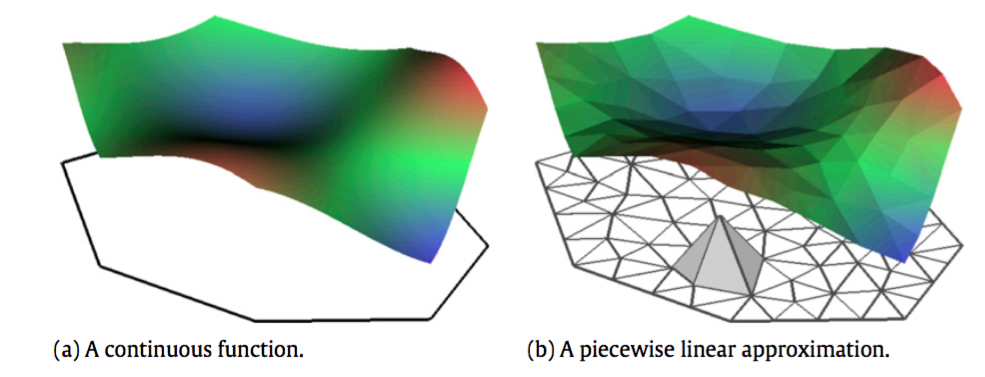
\includegraphics[scale=.4]{Images/PLBF.jpg}
	\caption{A Gaussian Markov random field, defined as the piecewise linear basis function $  x(\pmb{s}) = \sum_{k=1}^{n} \protect\psi_{k}(\pmb{s})x_{k}$, approximates a Matern GRF. This image illustrates how a triangular mesh over the domain determines basis functions $\protect\psi_{k}(\pmb{s})$ 
	\citep{Simpson2012}.}
	\end{figure}
	
Keep in mind that a realization of a GRF is essentially a function, and Figure 12 shows how a discrete piecewise linear basis function can approximate a continuous function \citep{Simpson2012}. We have $\psi_{k}(\pmb{s}) = 1$ at the $k\text{th}$ vertex, $0$ at all other vertices, and surface function values for triangle interior points are linear combinations of the three home triangle vertices.

\subsubsection{GMRF Weights}

Stochastic calculus identities provide a way to calculate the weights in the basis representation. Define $\langle f, g \rangle = \int f(\pmb{u}) g(\pmb{u}) d\pmb{u}$, and find weights $\pmb{x}$ such that
$$ \left[ \left< \phi_{k}, (\kappa^{2} - \Delta)^{\alpha/2} \pmb{x} \right> \right]_{k = 1, \hdots, n} \overset{D}{=} \Big[ \langle \phi_{k}, \mathcal{W} \rangle \Big]_{k = 1, \hdots, n},$$
for a set of test functions $\phi_{k}$ \citep{Lindgren2011}. The appropriate weight vector $\pmb{x}$ gives the stochastic weak solution solution to the SPDE \citep{Mao2007}, \cite{Lindstrom2014}; we use the Galerkin solution, with $\alpha = 2$ and $\phi_{i} = \psi_{i}$ \citep{Lindgren2011}. Replace $\pmb{x}$ with basis function representation $\Sigma_{k}\psi_{k}w_{k}$,
$$ \left[ \left< \phi_{i}, (\kappa^{2} - \Delta)^{\alpha/2} \psi_{j} \right> \right]_{i,j}\pmb{w} \overset{D}{=} \Big[ \langle \phi_{k}, \mathcal{W} \rangle \Big]_{k}, $$
and let $\alpha = 2$ and $\phi_{i} = \psi_{i}$ as in the Galerkin solution:
$$ \Big(
\kappa^{2} [ \langle \psi_{i}, \psi_{j} \rangle ] + [ \langle \psi_{i}, -\Delta \psi_{j} \rangle ]
\Big) \pmb{w} \overset{D}{=} \Big[ \langle \psi_{k}, \mathcal{W} \rangle \Big]. $$
Let $\pmb{C}_{i,j} = \langle \psi_{i}, \psi_{j} \rangle$, and $ \pmb{G}_{i,j} = \langle \psi_{i}, - \Delta \psi_{j} \rangle$, so that
$$ \left(
\kappa^{2} \pmb{C} + \pmb{G} \right) \pmb{w} \overset{D}{=} N(\pmb{0},\pmb{C}).$$
For $\pmb{w} \sim N(\pmb{0}, \pmb{Q}^{-1})$, we have then
$$\pmb{Q}_{\kappa} = \left( \kappa^{2} \pmb{C} + \pmb{G} \right)^{T} \pmb{C}^{-1} \left( \kappa^{2} \pmb{C} + \pmb{G} \right).$$ 
However, $\pmb{C}_{ij}^{-1}$ has a sparse precision matrix, so replace $\pmb{C}$ with diagonal matrix $\widetilde{\pmb{C}}$,
$$ \widetilde{\pmb{C}}_{i,i} = \langle \psi_{i}, \pmb{1} \rangle = \int \psi_{i}(\pmb{s}) d\pmb{s}.$$ 
Note that this solution provides the distribution of the weights $x_{k}$, not $x(\pmb{s})$ itself, in the basis representation
$$ x(\pmb{s}) = \sum_{k=1}^{n} \psi_{k}(\pmb{s})x_{k}.$$
With this representation achieved, via the SPDE link, we move on to the approximation procedure that we aim for.

\subsection{Integrated Nested Laplace Approximations (INLA)}

INLA proceeds through a carefully constructed and calibrated series of calculations and approximations, to acheive estimates of key quantites. These quantites include the maginal posterior distributions for latent field parameters, $p(x_{i}|\pmb{y})$; and covariance hyperparameter posterior $p(\theta|\pmb{y})$. This means we never obtain posteriors $p(\pmb{x}|\pmb{y})$ and $p(\pmb{x},\pmb{\theta}|\pmb{y})$. 

\subsubsection{Step 1, Gaussian Approximation} % ======= ======

The basic approach to estimating $p(\pmb{x}|\pmb{\theta}, \pmb{y})$ is ``matching the mode and curvature at the mode'' of estimator $p_{G}(\pmb{x}|\pmb{\theta}, \pmb{y})$ to that of $p(\pmb{x}|\pmb{\theta}, \pmb{y})$ \citep{Rue2005}. As mentioned, INLA requires Gaussian priors for all paramters except covariance hyperparameters; but, INLA also requires conditional independence, whereby $p(\pmb{y}|\pmb{x}, \pmb{\theta}) = \prod_{i} p(y_{i}|\pmb{x}_{i},\pmb{\theta})$. Our analysis satisfies this necessity, and therefore $$p(\pmb{x}|\pmb{\theta},\pmb{y}) \propto \text{exp}\left(-\frac{1}{2}\pmb{x}^{T}\pmb{Q x} + \sum_{i} \text{log }p(y_{i}|\pmb{x}_{i},\pmb{\theta}) \right).$$ The Gaussian approximation takes the form
$$p_{G}(\pmb{x}|\pmb{\theta},\pmb{y}) \propto \text{exp} \left( -\frac{1}{2}(\pmb{x-\mu})^{T} (\pmb{Q} + \text{diag}(\pmb{c}) ) (\pmb{x - \mu}) \right),$$
where vectors $\pmb{c}$ and $\pmb{\mu}$ depend on second order Taylor expansions of $f(\pmb{x}) = \sum_{i} \text{log }p(y_{i}|\pmb{x}_{i},\pmb{\theta})$ about the mode \citep{Lindstrom2014}. A Newton-Raphson algorithm iteratively computes the mode and precision matrix until convergence \citep{Rue2009}. Step 2 uses this Gaussian approximation, $p_{G}(\pmb{x}|\pmb{\theta},\pmb{y})$.

\subsubsection{Step 2, Laplace Approximation}  % ====== ======

This step begins with two sides of a familiar identity, and its subsequent rearrangement.
\begin{align}
p(\pmb{y} , \pmb{x} | \pmb{\theta}) = p(\pmb{y} | \pmb{x}, \pmb{\theta}) p(\pmb{x} | \pmb{\theta})  &= p(\pmb{x} | \pmb{y}, \pmb{\theta}) p(\pmb{y} | \pmb{\theta}) \\
p(\pmb{y} | \pmb{x}, \pmb{\theta}) p(\pmb{x} | \pmb{\theta}) &= p(\pmb{x} | \pmb{y}, \pmb{\theta}) p(\pmb{y} | \pmb{\theta}) \\
\frac{p(\pmb{y} | \pmb{x}, \pmb{\theta}) p(\pmb{x} | \pmb{\theta})} {p(\pmb{x} | \pmb{y}, \pmb{\theta})} &= p(\pmb{y} | \pmb{\theta})  
\end{align}
We use this formulation of $p(\pmb{y} | \pmb{\theta})$ next, in the familiar Bayesianian proporionality.
\begin{align}
p(\theta|\pmb{y}) & \propto p(\pmb{y}|\pmb{\theta})p(\pmb{\theta}) \\
& \propto \frac{p(\pmb{y} | \pmb{x}, \pmb{\theta}) p(\pmb{x} | \pmb{\theta})}{p(\pmb{x} | \pmb{y}, \pmb{\theta})} \cdot p(\pmb{\theta})
\end{align}

For a given $\pmb{\theta}$, let $\pmb{x}_{0} = \text{argmax}_{x}p(\pmb{x}|\pmb{y},\pmb{\theta})$. Then,
$$ p(\pmb{\theta}|\pmb{y}) \approx \tilde{p}(\pmb{\theta}|\pmb{y}) \propto  \frac{p(\pmb{y} | \pmb{x}_{0}, \pmb{\theta}) p(\pmb{x}_{0} | \pmb{\theta})}{p_{G}(\pmb{x}_{0} | \pmb{y}, \pmb{\theta})} \cdot p(\pmb{\theta}),$$
where the Taylor approximation of $f(\pmb{x}) = \sum_{i} \text{log }p(y_{i}|x_{i})$, in $p_{G}(\pmb{x} | \pmb{y}, \pmb{\theta})$, expands about $\pmb{x}_{0}$. This approximation matches \cite{Tierney1986} Laplace approximation.  Then, we have approximate maximum likelihood estimate $\hat{\pmb{\theta}}_{\text{ML}} \approx \text{argmax}_{\theta} \tilde{p}(\pmb{\theta}|\pmb{y})$.

\subsubsection{Step 3, Numerical Integration} % === === === === ===
Numerical Integration over $\pmb{\theta}$, or elements of $\pmb{\theta}$, gives $p(x_{i}|\pmb{y})$ and $p(\theta_{i}|\pmb{y})$.
        $$ p(x_{j} | \pmb{y}) \approx \int p_{\text{G}}(x_{j}|\pmb{\theta, y})\tilde{p}(\pmb{\theta}|\pmb{y}) d\pmb{\theta} $$
        $$ p(\theta_{k} | \pmb{y}) \approx \int \tilde{p}(\pmb{\theta}|\pmb{y}) d\pmb{\theta}_{-k} $$

In summary, from a continuous domain the SPDE-INLA approxmation procedure provides, with improved speed, posterior estimates for $p(\pmb{\theta}|\pmb{y})$, $p(\theta_{i}|\pmb{y})$, and $p(x_{i}|\pmb{y})$. The R package \verb|INLA| implements this procedure, with flexible SPDE specifications for domain triangulation.

\subsection{Bayesian Inference in R-INLA}